\documentclass[
	tikz,
	11pt,
	border=10pt
	]{standalone}
%\documentclass[a4paper]{article}

\usepackage{tikz}
\usetikzlibrary{mindmap}

\pgfdeclarelayer{background}
\pgfdeclarelayer{foreground}
\pgfsetlayers{background,main,foreground}

\begin{document}

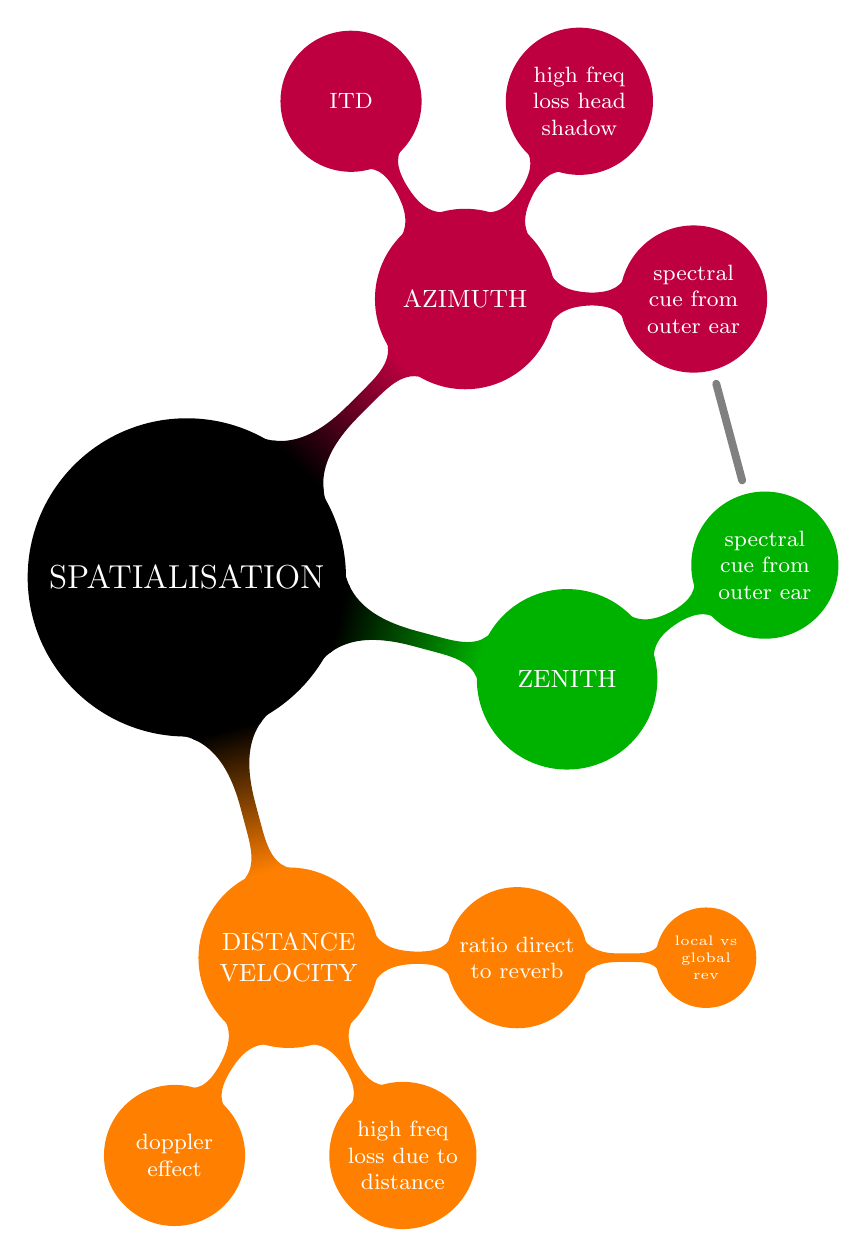
\begin{tikzpicture}
	\path[mindmap,concept color=black,text=white]
	node[concept] {SPATIALISATION}
		[clockwise from=45]
		child[concept color=purple] {
		node[concept] (azi) {AZIMUTH}
		[clockwise from=120]
	    child { node[concept] (itd) {ITD} }
		child { node[concept] (hfl) {high freq loss head shadow} }	
		child { node[concept] (asc) {spectral cue from outer ear} }				
	}
    child[concept color=green!70!black] {
		node[concept] (zen) {ZENITH}
		[clockwise from=30]
		child { node[concept] (zsc) {spectral cue from outer ear} }
    }
	child[concept color=orange] {
    	node[concept] (dis) {DISTANCE VELOCITY}
		[clockwise from=0]
	    child { node[concept] (rdr) {ratio direct to reverb}
	    	[clockwise from=0]
	    	child { node[concept] (lvg) {local vs global rev} }
		}
		child { node[concept] (hfl) {high freq loss due to distance } }
		child { node[concept] (hfl) {doppler effect } }		
	};

\begin{pgfonlayer}{background}
	\draw [concept connection]  (asc) edge (zsc);
\end{pgfonlayer}

\end{tikzpicture}

\end{document}
